% ============================================================================
% PINNing a Transformer: Two Physics-Injection Mechanisms for
% Hyperspectral Mineral Classification
%
% Target venue: PNAS Research Report (~6 pages, ~4,000 words main text,
%   ≤250-word abstract, 50–120-word Significance Statement, ~4 figures/tables,
%   ≤50 references).
%
% This is a pre-submission draft. PNAS production uses the official
% pnas-new.cls template; for now we use article + clean settings so the
% prose is editable. Reformat to the PNAS template before submission.
%
% Path setup:
%   \graphicspath points to ../Dissertation_images/ (shared with paper +
%     dissertation; figures already exist for Fig 1 and Fig 2).
%   \bibliography points to ../PaperofPartII/references (avoids divergence;
%     copy references.bib here later if PNAS requires self-contained submit).
% ============================================================================

\documentclass[11pt]{article}

\usepackage[T1]{fontenc}
\usepackage[utf8]{inputenc}
\usepackage{lmodern}
\usepackage[letterpaper, margin=1in]{geometry}
\usepackage{amsmath, amssymb, mathtools}
\usepackage{bm}
\usepackage{microtype}
\usepackage{hyperref}
\usepackage{graphicx}
\usepackage[table]{xcolor}
\usepackage{enumitem}
\usepackage{caption}

\graphicspath{{../Dissertation_images/}}

\newcommand{\R}{\mathbb{R}}
\DeclareMathOperator{\diag}{\mathrm{diag}}
\DeclareMathOperator{\argmax}{arg\,max}

\title{PINNing a Transformer: Physics-Informed Attention for Hyperspectral Mineral Classification}

\author{%
Kelli McCoy\thanks{Corresponding author: \texttt{kjm\_422@usc.edu}; ORCID: \textcolor{red}{TODO}}\\
Roger Ghanem\\
\\
\textit{Department of Civil and Environmental Engineering,}\\
\textit{Viterbi School of Engineering,}\\
\textit{University of Southern California, Los Angeles, CA 90089, USA}
}
\date{}

\begin{document}

\maketitle

% ============================================================================
% SIGNIFICANCE STATEMENT  (PNAS-required; 50–120 words; broad audience)
% ============================================================================
\section*{Significance Statement}
\noindent
Using hyperspectral imagery from orbiting remote-sensing platforms to identify surface materials and their abundances requires computationally intensive atmospheric correction and downstream spectral-library matching.
However, a cross-attention spectral transformer trained directly on top-of-atmosphere reflectance can serve as a low-latency surrogate for mineral identification, using a single forward pass.
The architecture creates a transparent path for adding established physical knowledge.
The result is an efficient framework for physics-informed transformers that supports faster ground processing, onboard screening, and revisit decision support for space-based applications.

% ============================================================================
% ABSTRACT  (≤250 words, single paragraph)
% ============================================================================
\section*{Abstract}
\noindent
Hyperspectral imaging spectrometers, particularly those operating in the visible shortwave infrared (VSWIR) range, enable quantitative remote-sensing measurement of surface composition.
Different materials leave distinct signatures in the reflected-light spectrum, from which their identity and abundance can be inferred.
NASA's Earth Surface Mineral Dust Source Investigation (EMIT) maps arid-region surface mineralogy with 285-band imaging spectroscopy. 
Operational data products require atmospheric correction and spectral-library matching before mineral identification. 
This paper presents a cross-attention transformer that predicts mineral labels directly from uncorrected top-of-atmosphere (TOA) reflectance, providing a post-hoc surrogate for the L1B-to-mineral ID classification at inference time.
The architecture treats each pixel spectrum as a wavelength-indexed sequence and uses learned query vectors to pool spectral evidence across bands. 
Two physics-injection mechanisms are evaluated within this attention architecture: spectroscopic priors, implemented as per-head attention-bias initialization from laboratory diagnostic wavelengths or USGS reference spectra, and statistical-invariance regularization, implemented as a consistency loss under label-preserving illumination and smooth spectral-slope perturbations. 
The best physics-prior configuration improves top-1 validation accuracy relative to the 8-head transformer-only baseline, while lower-capacity manual priors recover comparable accuracy with reduced training cost.
Attention analysis shows that the model emphasizes visible and near-infrared regions associated with Fe$^{3+}$ absorption structure, although attention weights are interpreted as diagnostic rather than causal explanations. 
Cross-region and full-granule experiments reveal a tradeoff: spectral priors improve top-1 accuracy, interpretability, and rare-class behavior (especially at constrained capacity), whereas statistical-invariance regularization's effect is concentrated in rare-class sensitivity rather than uniformly improving top-1 accuracy. 
These results demonstrate that physics-informed attention can provide efficient, interpretable surrogates for elements of hyperspectral mineral-retrieval pipelines.
\vspace{1em}
\noindent

\textbf{Keywords:}  physics-informed cross-attention$\vert$ hyperspectral imaging $\vert$ mineral classification $\vert$ statistical invariance $\vert$ spectral prior  


% ============================================================================
% 1. INTRODUCTION  (~700 words)
% ============================================================================
\section{Introduction}

Mineral dust suspended in the atmosphere is one of the largest sources of uncertainty in regional climate radiative-forcing predictions \cite{ipcc_2021}.
Light-colored airborne minerals scatter sunlight, while iron-bearing minerals absorb it and warm the atmospheric column; 
current climate models rely on uncertain estimates of iron-oxide abundance and can produce radiative-forcing predictions that vary by up to 460\% across plausible compositions \cite{emit_l1b_atbd}.
NASA's Earth Surface Mineral Dust Source Investigation (EMIT) was launched in 2022 to reduce this uncertainty by mapping arid-region surface mineralogy, producing approximately 1.6-million-pixel granules across 285 spectral bands.
Translating this data stream into operational mineral-identification products is therefore both a scientific and computational challenge.

The standard mineral-identification pipeline applied to EMIT and similar imaging-spectroscopy missions is a multi-stage sequence of per-pixel operations: atmospheric correction through radiative-transfer-model (RTM) inversion, followed by spectral-library matching against curated laboratory reference spectra.
Operational implementations rely on optimization-based schemes such as the Imaging Spectrometer Optimal Fitting (ISOFIT) inversion, often accelerated by neural-network RTM emulators \cite{thompson2018, brodrick2021}, before downstream mineral identification is performed.
Beyond the per-pixel computational cost, the staged architecture imposes operational latency.
EMIT mineral products are delivered with a two-month median latency from acquisition \cite{emit_l2b_atbd}, reflecting downlink, ingest, queueing, atmospheric correction, mineral matching, quality control, and archive production.
For petabyte-scale missions or time-sensitive applications such as volcanic-ash mapping, post-fire debris characterization, and dust-storm response, this operational delivery cycle becomes a constraint and burden separate from the cost of any single per-pixel computation.

This paper proposes an alternative paradigm: \emph{post-hoc direct retrieval with physics-informed injection} (Figure~\ref{fig:data_levels}).
Rather than executing the RTM-based atmospheric-correction and spectral-matching chain at inference time, a learned model is trained on a comparitively small set of previously processed L1B--L2B pairs and then used as a low-latency surrogate for the operational L1B-to-mineral ID mapping.
The model does not produce an atmospherically corrected reflectance product, nor does it claim independent mineral truth; 
its supervision is inherited from the operational science-data-system labels.
Its value is instead operational and methodological: after the one-time training cost, inference requires only a single forward pass from top-of-atmosphere (TOA) reflectance to mineral class.
This enables fast screening or mineral-label prediction without invoking the RTM during deployment.

\begin{figure}[!htbp]
\centering
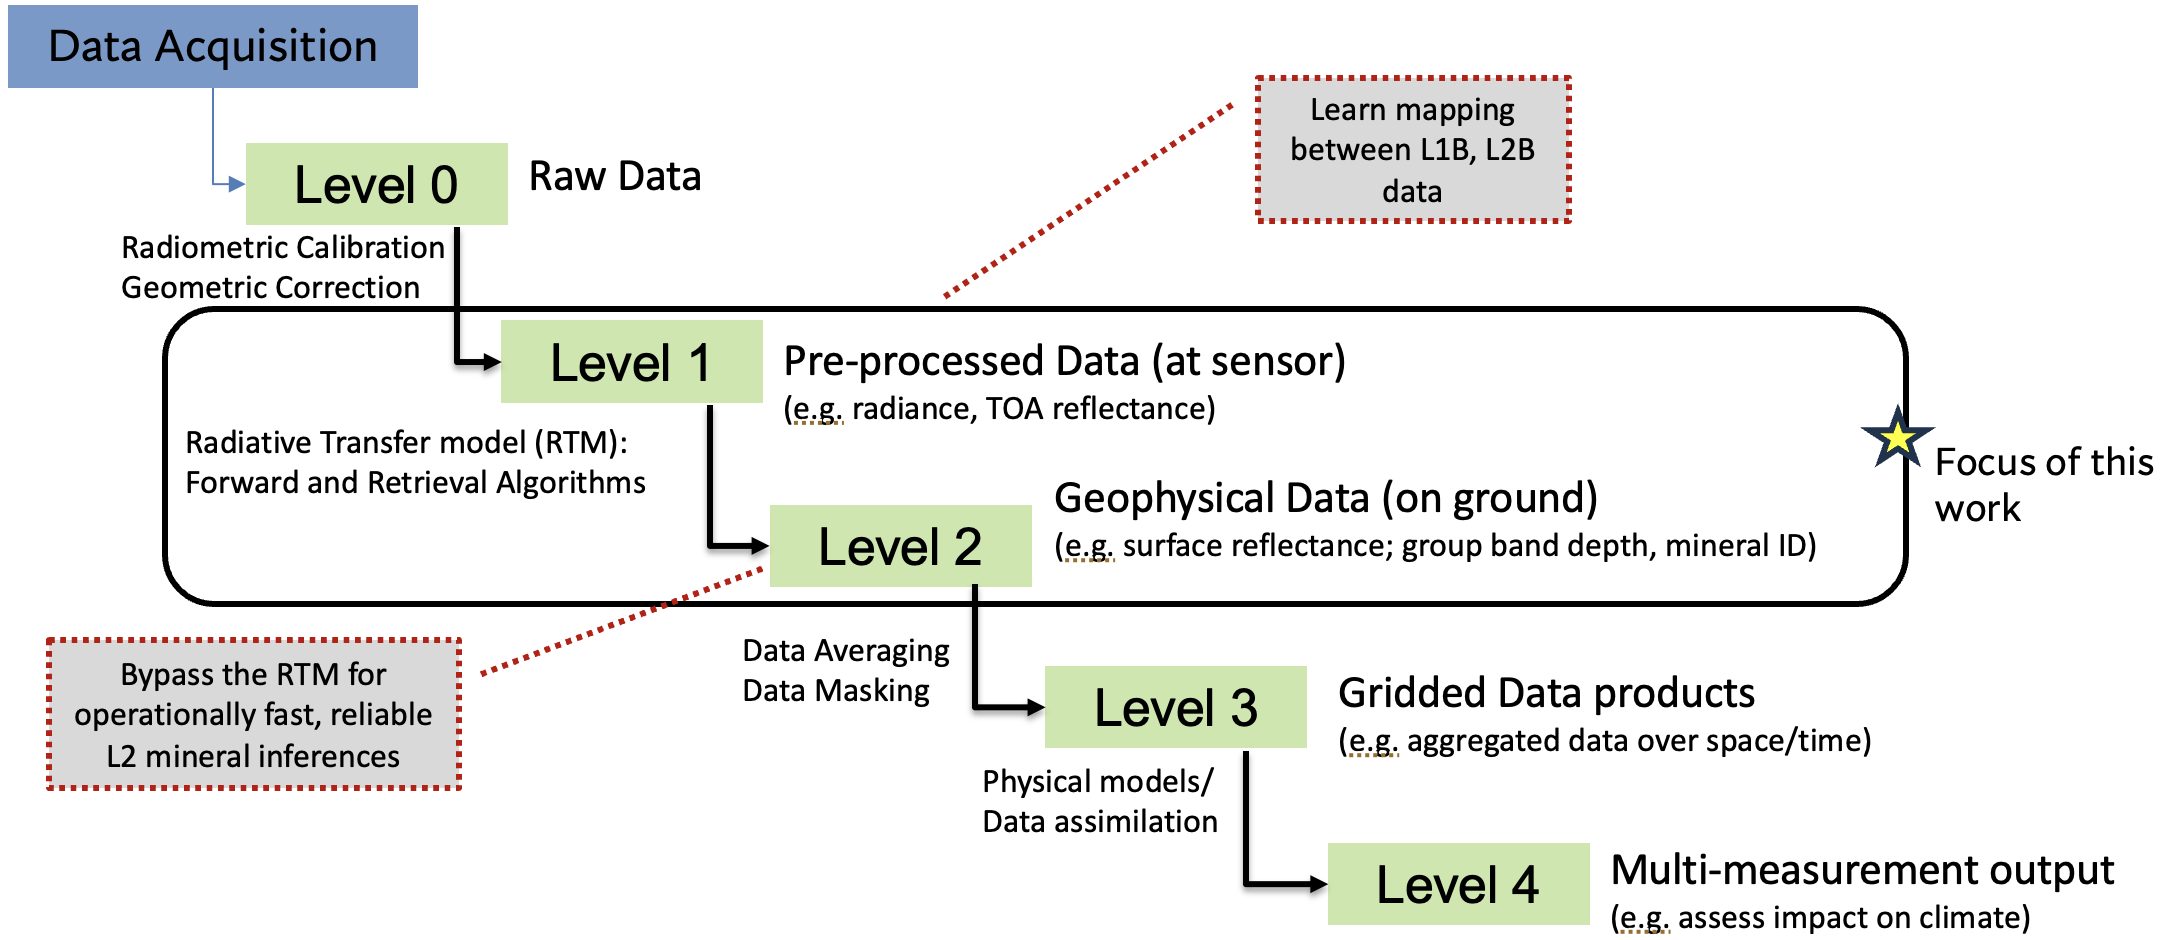
\includegraphics[width=\textwidth]{Data_level_depiction.png}
\caption{EMIT Science Data System (SDS) processing chain with the proposed post-hoc direct retrieval callout. The SDS performs per-pixel atmospheric correction (L1B$\to$L2A via ISOFIT optimal estimation and sRTMnet) followed by per-pixel spectral-library matching (L2A$\to$L2B via Tetracorder); 
the proposed approach maps L1B TOA reflectance directly to a mineral-class probability distribution in a single forward pass, after a one-time training cost on operational L1B--L2B pairs.}
\label{fig:data_levels}
\end{figure}

This direct TOA formulation is challenging because the model must infer mineralogical structure from spectra in which the surface signal is mixed with atmospheric scattering, absorption, transmission, illumination geometry, and sensor effects.
A purely data-driven model may learn useful spectral structure, but it may also exploit scene-specific shortcuts that do not transfer across regions.
The question addressed here is therefore not simply whether a transformer can classify EMIT spectra, but how physical knowledge should enter an attention-based model trained on operational remote-sensing products.
This question is studied through two physics-injection mechanisms: one architectural and one loss-based.

The cross-attention transformer presented here draws on the physics-informed and theory-guided machine-learning literature \cite{karpatne2017tgds, raissi2019pinn}.
Spectroscopic knowledge enters through the per-head attention bias $\bm{\beta}_h$, which can be initialized from known Fe$^{3+}$ diagnostic wavelengths or from principal components of EMIT-resampled USGS reference spectra.
Statistical-invariance knowledge enters through a consistency loss adapted from Vapnik \cite{vapnik2020}, which encourages predictions to remain stable under label-preserving TOA perturbations representing illumination scaling and smooth spectral-slope variation.
These mechanisms do not impose a hard radiative-transfer constraint and do not assume that TOA reflectance equals surface reflectance.
Instead, they provide controlled ways to test how spectroscopic priors and atmospheric invariance affect a learned post-hoc retrieval surrogate.

The approach is demonstrated on EMIT TOA hyperspectral observations for 95 Group~1 mineral classes.
The transformer learns Fe$^{3+}$-relevant spectral structure directly from data, with attention concentrating near visible and near-infrared regions associated with iron-oxide absorption.
Spectral-prior initialization improves top-1 accuracy, interpretability, and capacity efficiency, with the magnitude depending on head count and prior construction; statistical-invariance regularization's effect is concentrated in rare-class sensitivity rather than uniformly improving top-1 accuracy.
Together, these results position physics-informed attention as a practical mechanism for accelerating and interpreting the hyperspectral mineral-identification pipeline.

% ============================================================================
% 2. RESULTS  (~1500 words target; structure + TODO markers)
% ============================================================================
\section{Results}

A 4 and 8-head transformer baseline are trained on 1.26~million class-balanced TOA pixels from 396 EMIT granules over Africa and the Middle East, using derivative tokenization, learned query vectors, and a zero-initialized \emph{trainable} attention bias $\bm{\beta}_h$. 
No spectroscopic prior and no statistical-invariance regularization were applied in this baseline. 
Physics-injection configurations are evaluated against this baseline.

\subsection{Cross-attention transformer learns spectral structure from TOA reflectance}

A cross-attention transformer with $H$ learned query vectors that probe an $L=285$-band spectral token sequence. 
Each head produces a per-pixel attention vector, $\mathbf{A}_h \in \R^L$.
Figure~\ref{fig:trans4_attn} compares class-conditional mean attention for hematite and goethite at $H=4$ across four parameter-matched configurations: transformer-only, manual spectral prior, PCA-curated prior, and a Learning Using Statistical Invariants (LUSI) consistency loss ~\cite{vapnik2020}. 
These two endmember classes perform well on the held-out validation split: the transformer baseline reaches F1-score $0.93$ for hematite ($N=729$) and $0.92$ for goethite ($N=141$), substantially above the aggregate 95-class top-1 accuracy. 
The attention patterns show that the model emphasizes several wavelength neighborhoods physically plausible for ferric-mineral discrimination, but the learned peaks are not one-to-one matches to laboratory diagnostic wavelengths.

\begin{figure}[!htbp]
\centering
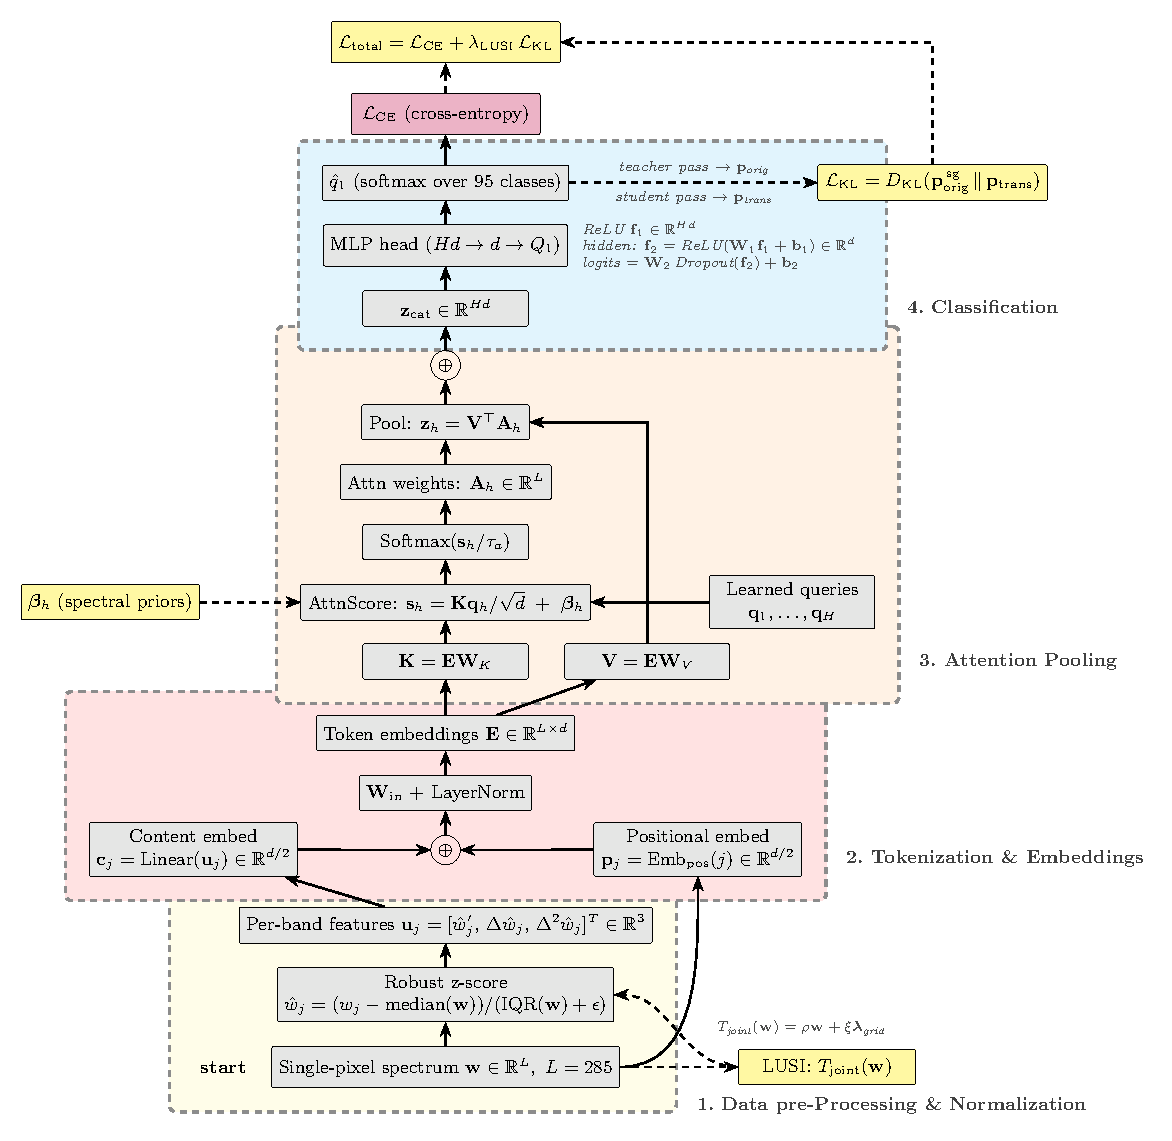
\includegraphics[width=\linewidth]{architecture.pdf}
\caption{End-to-end architecture overview. 
The forward pass is partitioned into four regions: preprocessing, tokenization, attention pooling, and classification. 
Spectral priors enter through the per-head attention bias $\bm{\beta}_h$; statistical-invariance regularization requires a second (student) forward pass through the network on a transformed input $T_{\text{joint}}(\mathbf{w})$, with the resulting prediction compared against the teacher prediction via a KL consistency loss.}
\label{fig:architecture}
\end{figure}

\begin{figure}[!htbp]
\centering
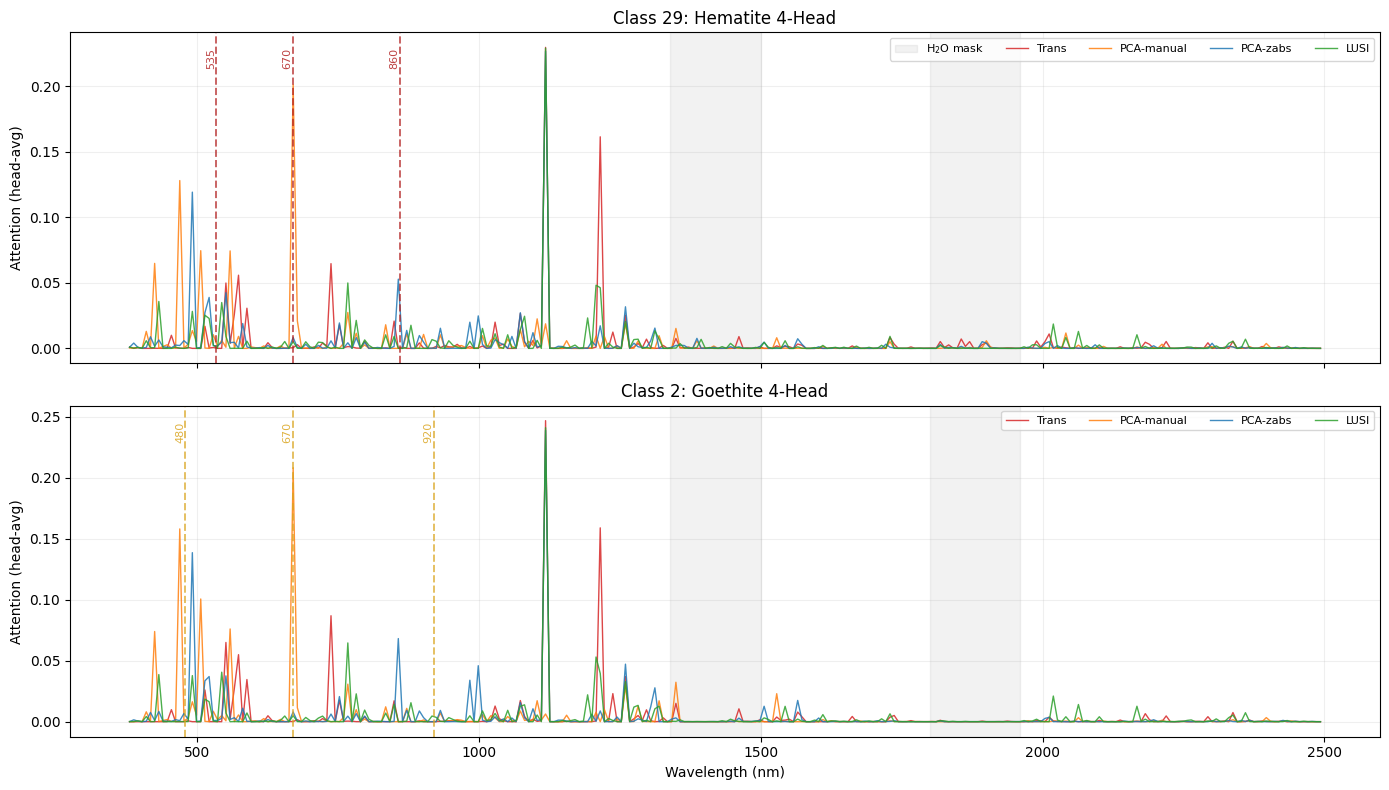
\includegraphics[width=\linewidth]{attention_headavg_compare4h.png}
\caption{Head-averaged class-conditional mean attention, $\bar{\mathbf{A}}^{(c)} \in \R^{285}$ for hematite (top) and goethite (bottom) at $H=4$. 
Curves compare the transformer baseline, manual Fe$^{3+}$ prior, PCA-curated prior, and LUSI configuration. 
Vertical dashed lines mark literature Fe$^{3+}$ diagnostic wavelengths for each mineral; light gray spans show H$_2$O atmospheric masks. 
The manual prior concentrates attention near canonical visible and VNIR ferric-iron regions, while the PCA-curated prior distributes attention over broader Fe-sensitive neighborhoods. 
The unguided transformer and LUSI configurations retain substantial attention at non-canonical wavelengths.}
\label{fig:trans4_attn}
\end{figure}

These attention results should not be read as a complete explanation of the final class decision.
Hematite and goethite often share the same attended wavelength neighborhoods because both are ferric-iron minerals.
Discrimination also depends on the value vectors $\mathbf{V} = \mathbf{E}\mathbf{W}_V$, which are learned linear projections of the token embeddings $\mathbf{E}$ (Fig.~\ref{fig:architecture}).
Each token combines normalized TOA reflectance with its first and second derivatives and a positional code, so the value vectors carry local slope and curvature information in addition to band magnitude.
Thus, attention identifies \emph{where} the model samples spectral evidence, while the downstream classifier separates minerals using both attention magnitudes and the wavelength-dependent content being pooled.

\subsection{Physics injection trades capacity, interpretability, and robustness}

\subsubsection{Spectral attention priors improve capacity efficiency at low head count}

Quantitative alignment between attention and USGS absorption-depth profiles supports the same interpretation.
At $H=4$, the manual and PCA-curated priors produce statistically significant head-averaged Spearman correlation with hematite and goethite absorption depth ($\rho \approx 0.17$--$0.24$), with per-head correlations reaching $\rho \approx 0.39$ ($p<10^{-7}$) where the prior anchors attention near canonical Fe$^{3+}$ regions.
The unguided $H=4$ transformer and LUSI-only configurations show no significant alignment, but at $H=8$ the unguided transformer rediscovers Fe$^{3+}$-consistent structure ($\rho=0.32$, $p<10^{-6}$), indicating that sufficient attention capacity recovers spectroscopic alignment without explicit initialization..

The attention bias $\bm{\beta}_h$ provides an explicit interface for architectural physics injection. 
Two spectroscopic initializations were evaluated. 
The manual prior places weak Gaussian bumps at literature Fe$^{3+}$ diagnostic wavelengths (480, 535, 670, 860, and 920~nm). 
The PCA-curated prior uses z-scored absolute principal-component loadings from a curated subset of EMIT-resampled USGS spectra, producing a broader reference-library variance prior over ferric-mineral spectral structure. 
In all main ablations, the transformer baseline uses the same trainable attention-bias parameters initialized at zero, so improvements from the prior-bearing models are attributable to initialization rather than extra model capacity.

The full ablation, with train-region (Africa/Middle East) top-1 and top-3 accuracies for every configuration, is consolidated alongside the cross-region results in Table~\ref{tab:crossscene}. Training plus validation took 117--326 minutes per configuration on a single Apple M4 Max laptop using PyTorch MPS; LUSI configurations approximately double the wall-clock cost of non-LUSI ones because each training step performs an additional augmented forward pass.

A non-attention random-forest baseline on the same Group~1 split reaches top-1 accuracy $0.716$ and top-3 accuracy $0.922$, while the unguided $H=4$ transformer reaches $0.789$ top-1 before any physics-informed mechanism is applied.
Thus, learned cross-attention provides a substantial gain over a conventional non-attention classifier. 
The architectural prior then improves the low-capacity transformer further: at $H=4$, the manual prior improves top-1 accuracy from $0.789$ to $0.808$, and the PCA-curated prior reaches $0.809$. 
These gains recover roughly two-thirds of the improvement obtained by doubling head count from $H=4$ to $H=8$ in the transformer-only model ($0.789 \rightarrow 0.819$), with no increase in model width or training time. 
This supports the capacity-efficiency interpretation: spectroscopic initialization helps a smaller transformer use its limited heads more productively.

At $H=8$, the story changes. 
The transformer-only baseline reaches $0.819$, the PCA-curated prior is essentially tied at $0.818$, and the manual prior falls to $0.806$. 
This suggests that priors help most when attention capacity is constrained. 
When capacity is larger, a narrow hand-coded prior can over-constrain the model, while a diffuse PCA prior is largely neutral because it overlaps more closely with the spectral structure the unguided model can discover from data.

The rare-class analysis further clarifies where the low-capacity prior helps. 
When per-class F1 is stratified by training-set support, the manual prior produces positive median F1 gain in every rarity bin, with the largest gains in the rare-but-learnable regime of roughly 200--2000 training pixels per class. 
The PCA-curated prior shows a similar positive median in this regime. 
By contrast, LUSI alone yields negative median F1 gain for rare classes, indicating that invariance regularization cannot substitute for class examples or spectroscopic information when the model must learn under limited support. 
Thus, the architectural prior is most useful as a sample-efficiency and capacity-efficiency tool, not as a universal replacement for model capacity.

Architectural and loss-based priors do not necessarily stack. 
At $H=4$, the combined PCA-curated  + LUSI configuration reaches top-1 accuracy $0.790$, statistically tied with the unguided baseline and below PCA-curated alone. 
This indicates interference between the two mechanisms at constrained capacity. 
A plausible explanation is that the consistency loss encourages the trainable bias to absorb differences between original and augmented passes, thereby distorting the structured spectral initialization. 
The two mechanisms therefore target different regimes: spectral priors improve in-distribution accuracy and interpretability under limited attention capacity, whereas statistical-invariance regularization tests robustness to label-preserving TOA perturbations but does not improve in-distribution top-1 accuracy in these experiments.

\subsubsection{Cross-region deployment reveals a robustness tradeoff rather than uniform top-1 improvement}

The LUSI-inspired consistency loss penalizes prediction drift under two label-preserving transformations of the input spectrum: multiplicative scaling, representing illumination variation, and a smooth additive spectral-slope change, representing low-order atmospheric or scattering-related slope variation.
These transformations are not a full atmospheric model and do not assume that TOA reflectance equals surface reflectance.
They are instead soft invariance predicates in TOA-input space.

\begin{table}[!htbp]
\centering
\small
\caption{Train-region (Africa/Middle East) and cross-region (SW US) accuracy for the locked configurations. Train columns report the held-out validation-pool accuracy on Africa/Middle East pixels. SW columns report the mean accuracy across 20 SW US granules each containing at least $20\%$ Group-1 mineral pixels, under full-granule inference. Pink rows mark the unguided transformer-only baselines at each head count; bold marks the leader within each head-count block on each SW metric.}
\label{tab:crossscene}
\begin{tabular}{p{0.24\linewidth}p{0.13\linewidth}p{0.13\linewidth}p{0.13\linewidth}p{0.13\linewidth}}
\hline
\rowcolor[gray]{0.85}
\textbf{Configuration} & \textbf{Train top-1} & \textbf{SW top-1} & \textbf{Train top-3} & \textbf{SW top-3} \\
\hline
\rowcolor{pink!30}
Trans 4H & 0.789 & 0.669 & 0.961 & 0.877 \\
\hline
\textbf{Manual 4H} & 0.808 & \textbf{0.724} & 0.967 & \textbf{0.919} \\
\hline
PCA-zabs 4H & 0.809 & 0.644 & 0.967 & 0.868 \\
\hline
LUSI 4H & 0.787 & 0.634 & 0.961 & 0.875 \\
\hline
\rowcolor{pink!30}
Trans 8H & 0.819 & 0.683 & 0.970 & 0.902 \\
\hline
Manual 8H & 0.806 & 0.699 & 0.966 & 0.896 \\
\hline
\textbf{PCA-zabs 8H} & 0.818 & \textbf{0.705} & 0.970 & \textbf{0.910} \\
\hline
LUSI 8H & 0.796 & 0.666 & 0.962 & 0.893 \\
\hline
\end{tabular}
\end{table}

Cross-region deployment to a geographically disjoint southwestern US desert region (20 mineral-populated granules) reduces top-1 accuracy by $8$--$17$ percentage points from the training-region validation pool, while top-3 accuracy stays in the $0.87$--$0.92$ range across all configurations (Table~\ref{tab:crossscene}). At $H = 4$ the manual prior leads cross-region (SW top-1 $= 0.724$, $-8.4$~pp drop), $+5.5$~pp above the unguided baseline and $+9.0$~pp above LUSI. At $H = 8$ the PCA-curated prior leads (SW top-1 $= 0.705$, $-11.3$~pp drop), narrowly above Manual 8H ($0.699$) and well above LUSI 8H ($0.666$). The 4H winner is the sharp manual prior; the 8H winner is the diffuse PCA-curated prior.

This sharp-vs-diffuse split at different head counts mirrors the in-distribution pattern visible in the train columns of Table~\ref{tab:crossscene}: narrow Gaussian bumps over-constrain attention at saturated capacity, while diffuse PCA loadings ($\sim$$220$ of $285$ bands) anchor better when more heads are available. The architectural priors are the consistent cross-region winners --- manual at constrained capacity, PCA-curated at saturated capacity. LUSI is last or next-to-last on both top-1 and top-3 at both head counts in this evaluation, providing no consistent cross-region top-1 or top-3 advantage.

\subsection{Post-hoc direct retrieval at deployment scale}
\label{sec:results_combined}

The operational value of the model is that inference requires a single forward pass from TOA reflectance to an SDS-equivalent mineral label. 
This does not replace atmospheric correction as a physical product, nor does it establish independent mineral truth. 
Rather, the model is a post-hoc surrogate for the operational L1B-to-mineral-product mapping learned from previously processed examples. 
Within that framing, the deployment question is whether validation-pool behavior persists when the model is applied to full EMIT granules.

Across three representative Africa/Middle East granules spanning approximately $1.4$--$1.6$ million mineral pixels each, the mean top-1 ordering is PCA-curated ($0.888$) $>$ Manual ($0.882$) $>$ Transformer ($0.874$) $>$ LUSI ($0.865$). 
This mirrors the validation-pool ordering among the $H=4$ configurations and confirms that architectural priors retain their in-distribution advantage at granule scale. 
Macro recall, which is sensitive to rare-class capture, favors architectural priors on every granule. 
For example, on one granule class~32 improves from F1 $=0.04$ under the transformer baseline to F1 $=0.32$ under the PCA-curated prior, despite having only 117 mineral pixels.

Cross-region full-granule inference is more difficult.
On the 20-granule southwestern US set, top-1 accuracy drops by $8$--$17$~pp across configurations (Table~\ref{tab:crossscene}), with the manual prior leading at $H = 4$ (SW top-1 $= 0.724$) and the PCA-curated prior leading at $H = 8$ (SW top-1 $= 0.705$).
The architectural priors are therefore the consistent cross-region winners --- manual at constrained capacity, PCA-curated at saturated capacity --- while LUSI is last or next-to-last on both top-1 and top-3 at both head counts.

Each full granule is processed in approximately 45~seconds on the same Apple M4 Max laptop used for training. 
This inference time is orders of magnitude shorter than the operational L2B product-delivery latency, although the two quantities are not directly comparable because operational latency also includes downlink, queueing, quality control, and archive production. 
The practical conclusion is that a physics-informed attention model can provide a fast, inspectable surrogate for mineral-label prediction, suitable for accelerated ground screening, onboard prioritization studies, and stress-testing where spectral priors or invariance assumptions help or hurt.

% ============================================================================
% 3. DISCUSSION  (~800 words target; TODO body)
% ============================================================================
\section{Discussion}

\paragraph{Physics injection as an experimental probe, not a universal improvement.}
The central result of this work is not that every physics-informed intervention improves every metric. 
Instead, the experiments show that attention architectures provide a controlled way to test \emph{how} physical knowledge enters a learned remote-sensing surrogate, and when that knowledge helps or constrains the model. 
The per-head attention bias $\bm{\beta}_h$ serves as an explicit architectural interface for spectroscopic priors, while the statistical-invariance loss provides an external constraint on the input--output mapping through label-preserving transformations. 
These two mechanisms instantiate two documented modes of physics-informed learning --- architectural prior initialization and loss-based regularization \cite{karpatne2017tgds,raissi2019pinn} --- but their empirical effects differ. 
Spectral-prior initialization improves capacity efficiency and interpretability when attention heads are limited, especially for rare classes and ferric-mineral endmembers. 
At larger head count, however, the unguided transformer can discover comparable Fe$^{3+}$-relevant structure directly from data, and narrow manual priors can over-constrain attention. 
Statistical-invariance regularization does not improve in-distribution top-1 accuracy in these experiments; its value is instead diagnostic, revealing a tradeoff between fitting the sampled training distribution and maintaining sensitivity to label-preserving spectral perturbations.

\paragraph{What the attention analysis does and does not prove.}
The attention maps provide spectroscopic evidence that the model emphasizes wavelength regions consistent with iron-oxide discrimination, including visible Fe$^{3+}$ charge-transfer structure and VNIR crystal-field regions. 
However, attention weights are not causal explanations by themselves. 
They indicate where each learned query samples the spectrum, while the final class decision also depends on the value vectors $\mathbf{V}_j$, which encode reflectance magnitude, local derivative structure, and band-position information. 
This distinction is particularly important for hematite and goethite, whose diagnostic features overlap substantially. 
The fact that both minerals share attention peaks is therefore not a failure of discrimination; it reflects shared ferric-iron spectral structure. 
The mineral-specific decision is made downstream by the classifier head using the content pooled from those regions. 
Thus, the appropriate interpretive claim is that the learned representation is \emph{consistent with} known spectroscopy, not that attention alone recovers the full physical retrieval logic.

\paragraph{Spectral priors improve efficiency under constrained capacity.}
The clearest benefit of the architectural prior appears at $H=4$, where both the manual Fe$^{3+}$ prior and the curated PCA prior recover much of the gain obtained by doubling the number of heads in the transformer-only baseline. 
This supports a capacity-efficiency interpretation: a weak spectroscopic initialization helps a smaller transformer allocate limited attention heads toward physically plausible regions of the spectrum. 
The rare-class analysis strengthens this conclusion. 
Architectural priors produce their largest gains in the rare-but-learnable regime, where there are enough examples to train a classifier but not enough for the model to reliably discover all discriminative spectral structure from data alone. 
This behavior is consistent with the broader expectation from physics-informed and theory-guided learning that domain knowledge is most valuable when data or capacity are constrained. 
The $H=8$ results qualify the claim: once attention capacity is sufficient, a sharp manual prior can become a liability, while a broader PCA-derived prior is closer to neutral. 
The practical implication is that physics priors should be treated as tunable inductive biases, not fixed truths.

\paragraph{Statistical-invariance regularization reveals a robustness tradeoff.}
The LUSI-inspired consistency loss was designed to encourage stability under illumination scaling and smooth spectral-slope perturbations. 
These transformations are not a substitute for atmospheric correction and do not assume that TOA reflectance equals surface reflectance. 
They are soft label-preserving predicates in TOA-input space, motivated by the observation that mineral identity should be stable under moderate brightness and low-order continuum variation. 
The empirical results show that this regularization does not improve in-distribution top-1 accuracy and can reduce it, especially when capacity is limited. 
This is not unexpected: an invariance penalty restricts the admissible function class and can suppress useful scene-specific cues. 
Its benefit is more apparent in robustness-oriented metrics, principally macro-recall, where the loss encourages the model to rely less on brittle spectral-scale and slope information.
The main conclusion is therefore not that LUSI is the best classifier, but that statistical-invariance regularization exposes a different axis of performance than spectral-prior initialization: robustness and rare-class sensitivity rather than maximum in-distribution accuracy.

\paragraph{Post-hoc direct retrieval as an operational surrogate.}
The proposed model should be understood as a post-hoc surrogate for the operational L1B-to-mineral-product mapping, not as an independent physical retrieval of surface mineralogy. 
Its labels are inherited from the EMIT science data system, and its accuracy is therefore bounded by the quality, thresholds, and assumptions of the upstream atmospheric-correction and spectral-matching pipeline. 
Within that scope, the operational advantage is substantial: once trained, the model maps TOA reflectance to mineral labels using a single forward pass and does not invoke an RTM at inference. 
Full-granule experiments show that this inference can be performed on commodity Apple Silicon hardware in roughly tens of seconds per granule. 
This timing should not be directly compared to end-to-end operational product latency, which includes downlink, queueing, ingest, quality control, archive generation, and multi-stage ground processing. 
Nevertheless, the gap is operationally meaningful. 
A fast surrogate could support rapid ground screening, prioritization of scenes for full processing, onboard event detection, or exploratory analyses in which approximate mineral labels are useful before validated products are available.

\paragraph{Conditions for transfer beyond EMIT.}
The framework is transferable in structure, not in its specific spectral content. 
For another sensor, mineral group, or physical-science application, the diagnostic wavelengths, prior construction, and label-preserving transformations would have to be rebuilt from the relevant physics. 
What transfers is the recipe: identify a feature axis with physical meaning, encode prior knowledge as a weak learnable bias over that axis, and evaluate whether loss-based invariances improve robustness to known label-preserving transformations. 
In hyperspectral remote sensing, the feature axis is wavelength and the priors come from spectroscopy. 
In other domains, the analogous axis might be time, frequency, spatial scale, molecular position, or graph connectivity. 
This makes the approach most appropriate for problems where labels are expensive because they are generated by an upstream physical model or expert pipeline, and where domain knowledge specifies either diagnostic input regions or transformations that should preserve the label.

\paragraph{Limitations.}
Several limitations bound the present results. 
First, the labels are operational mineral-product labels, not independent field-validated mineral truth. 
The model therefore learns to emulate a science-data-system product and may inherit that product's biases. 
Second, the main ablation results are single-seed runs at one training-set scale; additional seeds and training-size sweeps are needed to quantify statistical variability and to test whether physics priors become more valuable in smaller-data regimes. 
Third, attention maps are diagnostic visualizations rather than causal explanations; ablation, masking, or counterfactual tests are needed to prove that specific bands drive individual decisions. 
Fourth, cross-region performance is evaluated here on a single deployment region (southwestern US) under full-granule inference, which preserves regional class imbalance, rare-class sparsity, and atypical mineral assemblages but may not generalize to all geographic settings.
Fifth, the LUSI perturbations are intentionally simple. 
The scale and slope-change transformations capture only low-order label-preserving effects and do not represent the full atmospheric radiative-transfer process.
Finally, the softmax outputs are model probabilities, not calibrated posterior probabilities; deployment would require calibration or uncertainty quantification to identify when the surrogate should defer to the operational pipeline.

\paragraph{Future work.}
The next step is to convert the surrogate from a promising research model into a validated operational aid. 
This requires independent validation against field or laboratory-confirmed mineral targets, cross-sensor testing on missions such as PRISMA, EnMAP, SBG, or CHIME, and systematic evaluation across aerosol optical depth, water-vapor burden, solar/view geometry, and surface-brightness regimes. 
A second direction is causal interpretability: band-masking, counterfactual spectral editing, and attention-bias intervention experiments could determine whether the wavelengths highlighted by attention are necessary for correct classification. 
A third direction is uncertainty quantification, including temperature scaling, conformal prediction, ensembles, or post-hoc calibration against operational confidence measures. 
A fourth direction is adaptive physics injection: instead of fixing manual or PCA priors, the model could learn when to trust, attenuate, or override a prior based on scene conditions. 
Finally, onboard or near-realtime deployment studies should evaluate not only inference speed, but also memory footprint, radiation-tolerant compute constraints, downlink prioritization value, and failure-detection logic for cases where the surrogate should defer to full ground processing.

% ============================================================================
% 4. MATERIALS AND METHODS  (~1000 words target)
% ============================================================================
\section{Materials and Methods}

The architectural overview is shown in Figure~\ref{fig:architecture}. 
The four shaded regions correspond to the base forward pass---preprocessing, tokenization, attention pooling, and classification---while the two side blocks correspond to optional physics-injection mechanisms: spectral-prior initialization of the attention bias and statistical-invariance consistency regularization. 
Full architectural equations, hyperparameters, data sanitization, and extended ablation results are provided in the SI Appendix.

\paragraph{Cross-attention transformer.}
Each pixel is represented by its $L=285$-band EMIT top-of-atmosphere (TOA) reflectance vector. 
Reflectance values are robust-z-score normalized using per-band medians and interquartile ranges computed from the training split only. 
The normalized spectrum is then tokenized using a shape-aware spectral representation that concatenates each band value with first and second finite differences along wavelength, following the derivative-spectroscopy motivation of Tsai and Philpot~\cite{tsai1998derivative}. 
Each spectral token is embedded together with a learned band-position embedding.

The model uses $H$ learned query vectors $\mathbf{q}_h \in \mathbb{R}^d$ to cross-attend to the $L$ spectral tokens. 
For head $h$, the attention score vector is
\[
\mathbf{s}_h
=
\frac{\mathbf{K}\mathbf{q}_h}{\sqrt{d}}
+
\bm{\beta}_h,
\]
where $\mathbf{K}$ is the key matrix and $\bm{\beta}_h \in \mathbb{R}^L$ is a learnable per-head spectral bias. 
The attention weights are
\[
\mathbf{A}_h
=
\mathrm{softmax}\left(\frac{\mathbf{s}_h}{\tau_a}\right),
\]
where $\tau_a$ is the attention temperature. 
The pooled head representation is
\[
\mathbf{z}_h = \mathbf{V}^{T}\mathbf{A}_h,
\]
and the $H$ pooled vectors are concatenated and passed to a two-layer MLP classifier that produces logits over $Q_1=95$ Group~1 mineral classes.

In the transformer-only baseline, $\bm{\beta}_h$ is initialized to zero but remains trainable. 
This makes the baseline parameter-matched to the physics-prior configurations: all models have the same attention-bias capacity, but only the physics-prior models receive spectroscopic information at initialization.

\paragraph{Architectural prior: attention-bias initialization.}
Spectroscopic prior information is injected by initializing $\bm{\beta}_h$ before training. 
The bias is not a hard constraint; after an optional short freeze period, it is updated by gradient descent like the rest of the model. 
Thus, the prior acts as a weak inductive starting point that the model can preserve, attenuate, amplify, or reshape.

Two prior constructions are evaluated. 
In the manual mode, literature-derived Fe$^{3+}$ diagnostic wavelengths are encoded as Gaussian bumps over wavelength. 
The default manual prior uses the visible and near-infrared ferric-iron regions: 480,\ 535,\ 670,\ 860,\ 920 nm.
corresponding to goethite and hematite visible features and broader Fe$^{3+}$ crystal-field absorption structure. 
Each center wavelength $\lambda_c$ is represented as
\[
b(\lambda;\lambda_c,\sigma)
=
\exp\left[
-\frac{(\lambda-\lambda_c)^2}{2\sigma^2}
\right],
\]
with $\sigma=25$~nm. 
The Gaussian bumps are assigned to heads by round-robin allocation and normalized before scaling by the prior strength $\alpha$.

In the PCA-curated mode, the prior is constructed offline from EMIT-resampled USGS reference spectra. 
The reference subset includes hematite and goethite targets, ferric oxide/hydroxide/sulfate confusers, and selected Fe-bearing hard negatives. 
Spectra are sanitized to remove fill values and non-finite entries, small missing gaps are interpolated along wavelength, and spectra with excessive missingness are excluded. 
Before PCA, each spectrum is row-normalized to reduce dominance by broadband albedo and emphasize spectral shape. 
Principal components are computed over valid non-water-vapor bands, expanded back to the full 285-band EMIT grid, and converted into attention-bias profiles using z-scored absolute loading magnitudes:
\[
\beta_h(\lambda)
=
z\left(|v_h(\lambda)|\right),
\]
where $v_h(\lambda)$ is the signed loading vector for component $h$. 
Water-vapor absorption regions and the noisy long-wavelength edge are set to zero in the prior.

\paragraph{Loss-based prior: statistical-invariance consistency regularization.}
The loss-based physics injection is implemented as a consistency regularizer motivated by Vapnik--Izmailov statistical invariants~\cite{vapnik2020}. 
For each training pixel, the model compares its prediction on the original spectrum with its prediction on a perturbed spectrum generated by two label-preserving transformations in TOA-input space.

The first transformation is a multiplicative scale factor $\rho \sim U(0.8,1.2)$, representing moderate illumination or topographic-brightness variation. 
The second is a smooth additive spectral-slope change $\xi \sim \mathcal{N}(0,0.01)$,
applied along the wavelength axis to represent low-order spectral-slope variation associated with residual atmospheric or scattering effects. 
These perturbations are not intended to perform atmospheric correction and do not assume that TOA reflectance equals surface reflectance. 
They are conservative label-preserving transformations: mineral identity should remain stable under moderate brightness and smooth-slope changes.
The joint transformation applied to a single-pixel spectrum $\mathbf{w}$ is
\[
T_{\text{joint}}(\mathbf{w}) = \rho\,\mathbf{w} + \xi\,\bm{\lambda}_{\text{grid}},
\]
where $\bm{\lambda}_{\text{grid}} \in \R^L$ is a fixed linear wavelength-axis vector (a ramp from $-1$ to $+1$ across the $L$ bands) and $\rho, \xi$ are sampled independently for each pixel at each training step.

The transformations are applied in raw reflectance space.
The normalized input is first denormalized, perturbed, clamped to a physically valid range, and then renormalized before being passed through the model. 
The unperturbed prediction acts as a stop-gradient teacher distribution, while gradients propagate through the perturbed student pass. 
The consistency loss is the temperature-scaled Kullback--Leibler divergence
\[
\mathcal{L}_{\mathrm{KL}}
=
D_{\mathrm{KL}}
\left(
\mathbf{p}_{\text{orig}}^{\mathrm{sg}}
\;\|\;
\mathbf{p}_{\text{trans}}
\right),
\]
where $\mathbf{p}_{\text{orig}}$ is the model prediction on the original spectrum, $\mathbf{p}_{\text{trans}}$ is the prediction on the transformed spectrum $T_{\text{joint}}(\mathbf{w})$, and superscript $\mathrm{sg}$ indicates stop-gradient: during training the clean-input prediction is treated as a fixed target so that gradients flow only through the perturbed-input prediction, preventing the degenerate solution in which both predictions drift toward a shared trivial output to make the loss artificially small.
The total objective is
\[
\mathcal{L}_{\mathrm{total}}
=
\mathcal{L}_{\mathrm{CE}}
+
\lambda_{\mathrm{LUSI}}\mathcal{L}_{\mathrm{KL}},
\]
with $\lambda_{\mathrm{LUSI}}=1$ when consistency regularization is enabled.

\paragraph{Training data.}
Training and validation use a class-balanced sample of 1{,}260{,}203 EMIT TOA pixels drawn from 396 granules over Africa and the Middle East. 
Each pixel is paired with the Group~1 mineral label assigned by the operational EMIT mineral-identification pipeline, which applies Tetracorder-style spectral matching to the pipeline's atmospherically corrected product~\cite{clark2003tetracorder}. 
The labels are therefore treated as operational science-data-system products rather than independent mineral ground truth.

The original Group~1 distribution is highly imbalanced and dominated by iron-bearing minerals, especially goethite and nano-hematite variants. 
To reduce dominance by the most common classes, a stratified per-class cap of 7{,}500 pixels is applied; the sampled dataset is then split 90/10 into training and validation sets using a fixed random seed. 
Labels with value zero are treated as unclassified and excluded before training; mineral labels 1--95 are shifted to class indices 0--94.

\paragraph{Optimization and ablation protocol.}
Models are trained for 120 epochs using AdamW with peak learning rate $5\times10^{-4}$, cosine decay, 5\% linear warmup, batch size 1{,}024, and cross-entropy loss with label smoothing $0.05$~\cite{szegedy2016rethinking}. 
The attention-bias parameters are placed in a separate optimizer group with zero weight decay. 
For prior-bearing models, the initialized prior heads are frozen for a short initial period and then released for standard gradient-based training. 
For transformer-only and LUSI-only baselines, the attention bias is initialized at zero and learned from data.

All ablation runs use the same data split, random seed, hardware, optimizer settings, and data pipeline. 
Wall-clock timings are measured on a single Apple M4 Max laptop using PyTorch's MPS backend. 
These timings are intended to compare configurations under identical workstation conditions, not to represent an optimized high-performance-computing deployment.

\paragraph{Attention and spectral-alignment analysis.}
Attention weights are averaged by class and by head to evaluate which wavelength regions the model emphasizes for selected minerals. 
For hematite and goethite, attention profiles are compared with literature diagnostic wavelengths and with EMIT-resampled USGS absorption-depth profiles. 
Spearman rank correlation between attention magnitude and absorption depth is used as a quantitative alignment diagnostic. 
These attention analyses are interpreted as evidence of spectroscopic consistency, not as causal explanations of individual predictions: the final class decision also depends on the value vectors and downstream classifier.

\paragraph{Cross-region evaluation.}
Cross-region evaluation applies trained checkpoints to complete granules from a geographically disjoint southwestern US desert region (20 granules each containing at least $20\%$ Group-1 mineral pixels) using the same Group~1 label set.
Reported values compare the mean per-granule top-1 accuracy on the southwestern US set with the same model's Africa/Middle East validation-pool accuracy (Table~\ref{tab:crossscene}).
Full-granule cross-region deployment preserves regional class imbalance and rare-class sparsity, which sampled-pixel cross-region tests do not.

\paragraph{Full-granule inference.}
Deployment-scale inference is evaluated by applying trained checkpoints to complete EMIT granules. 
For each granule, the model predicts a Group~1 mineral label for every valid mineral pixel, and predictions are compared with the operational Group~1 label product. 
Top-1 accuracy, top-3 accuracy, macro-F1, and macro-recall are reported. 
Macro-level metrics are included because they are more sensitive to rare-class behavior than aggregate top-1 accuracy. 
Full-granule inference is also used to measure practical runtime. 
On the Apple M4 Max workstation, full-granule inference takes approximately tens of seconds per granule, demonstrating that the learned surrogate can be evaluated far faster than the end-to-end operational product-delivery cycle, while acknowledging that operational latency includes downlink, queueing, quality control, and archive generation in addition to algorithmic computation.
% ============================================================================
% BACK MATTER (PNAS-required)
% ============================================================================
\section*{Acknowledgments}
\textcolor{red}{\textbf{TODO:} Funding sources, computing resources, reviewers thanked, etc.}

\section*{Author Contributions}
\textcolor{red}{\textbf{TODO:} Narrative or CRediT-style contributions for K.~McCoy and R.~Ghanem.}

\section*{Competing Interests}
The authors declare no competing interests.

\section*{Data and Software Availability}
Training and inference code, including the cross-attention transformer (release \texttt{r17}), the curated-PCA prior pipeline, and the manual-prior generator, is available at \url{https://github.com/kjm422/Dissertation-transformer}.
EMIT L1B TOA reflectance and L2B mineral-identification products are publicly available from the NASA LP DAAC (\url{https://lpdaac.usgs.gov/products/emitl1bradv001/}; \url{https://lpdaac.usgs.gov/products/emitl2bminv001/}).
USGS Spectral Library reference spectra are available at \url{https://crustal.usgs.gov/speclab/QueryAll07a.php} \cite{kokaly2017usgs}.
The mineral grouping matrix used to map Tetracorder identifications to Group-1 / Group-2 labels is included with the EMIT L2B product release.


% ============================================================================
% REFERENCES
% ============================================================================
\bibliographystyle{unsrt}
\bibliography{../PaperofPartII/references}

\end{document}
